\chapter{データセット}
既存の公開されている犬一人称視点動画データセットにDogCentric Actibity Dataset(DCAD)がある.
本研究ではレスキュー犬向けにラベル付けされたレスキュー犬訓練動画が必要であるため,本実験ではレスキュー犬の訓練動画を用いた.訓練動画を用いる前に,犬一人称視点動画から行動分類が可能かどうかを確認するため簡易な予備実験を行なった.予備実験にはDCADを用いた.

また,本実験には現在作成中のサイバーレスキュー犬の訓練データセットを用いた.

\section{DogCentric Activity Dataset (DCAD)}
4頭の犬の背中にGoProカメラを取り付けて散歩をした動画を単一クラス分けしたデータセット~図\ref{DCAD_img}.動画は320 x 240 解像度,48 frames per secondで撮影されている.散歩する地域やコースは犬毎に異なり,アノテーションはそれぞれの犬に同じラベルのアクティビティをラベル付けしている.
アクティビティは10クラス(
横断前の待機: Car, 水分の摂取: Drink, 手渡しでの食事: Feed, 左を向く: Look at left, 右を向く: Look at right, 人間が犬を撫でる: Pet, ボールで遊ぶ: Play with ball, 身体をブルブルと振る: Shake, 何かの匂いを嗅ぐ: Sniff, 歩く: Walk
)あり,それぞれ合わせて209クリップになる~表\ref{DCADlabel}.
\begin{table}[tb]
 \centering
 \caption{DogCentric Activity Dataset 内訳}\label{DCADlabel}
 \scalebox{1.00}[1.00]{
  \begin{tabular}{|l||c|c|c|c|c|c|c|c|c|c|}
   \hline \hline
   Activity& Car &Drink& Feed& Left&Right& Pet & Ball&Shake&Sniff&Walk \\ \hline
   Clips   &   26&   10&   25&   21&   17&   25&   14&   19&   27&   25\\ \hline
  \end{tabular}
 }

\end{table}

\begin{figure}[htbp]
%  \begin{center}
    \begin{tabular}{c}
     % 0
      \begin{minipage}{0.18\hsize}
        \begin{center}
          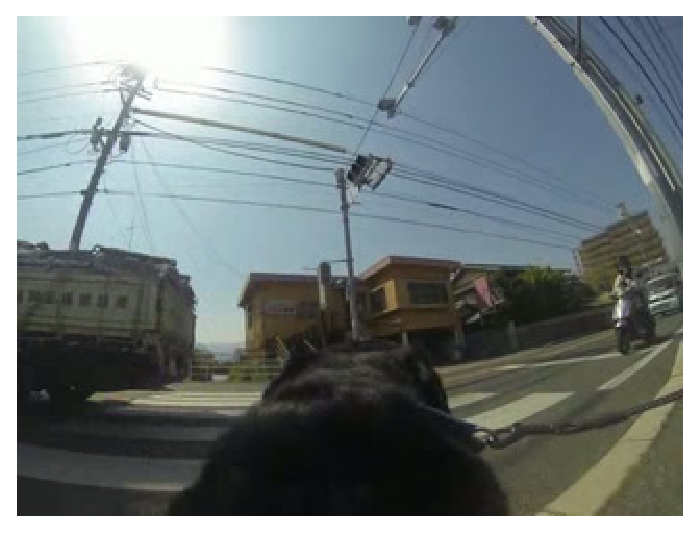
\includegraphics[clip, width=1.7cm]{./Figures/HC005.eps}
          \hspace{0.3cm} { }
        \end{center}
      \end{minipage}
      \begin{minipage}{0.18\hsize}
        \begin{center}
          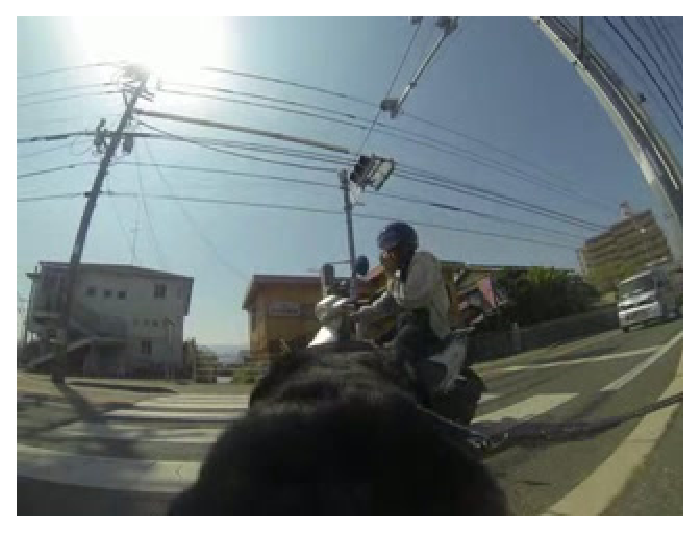
\includegraphics[clip, width=1.7cm]{./Figures/HC006.eps}
          \hspace{0.3cm} { }
        \end{center}
      \end{minipage}

      % 2
      \begin{minipage}{0.18\hsize}
        \begin{center}
          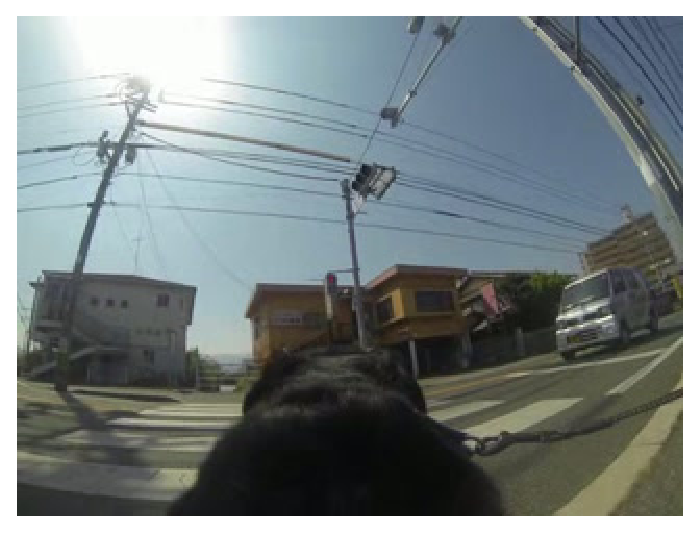
\includegraphics[clip, width=1.7cm]{./Figures/HC007.eps}
          \hspace{0.0cm} {Car}
        \end{center}
      \end{minipage}

      % 4
      \begin{minipage}{0.18\hsize}
        \begin{center}
          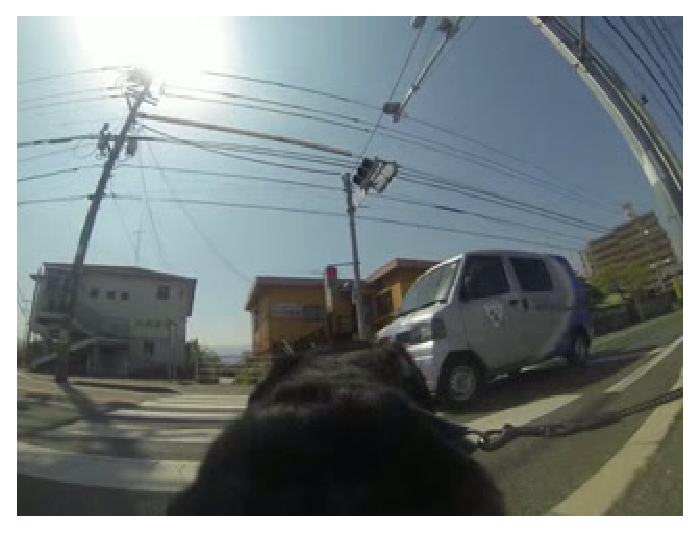
\includegraphics[clip, width=1.7cm]{./Figures/HC008.eps}
          \hspace{0.1cm} { }
        \end{center}
      \end{minipage}
      % 5
      \begin{minipage}{0.18\hsize}
        \begin{center}
          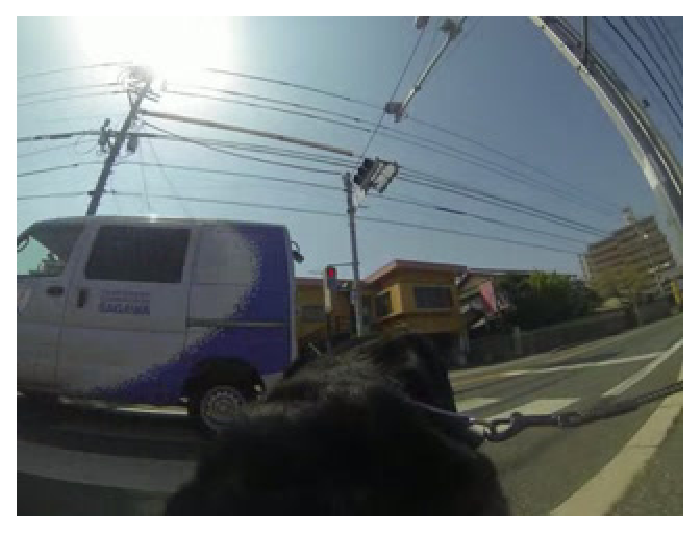
\includegraphics[clip, width=1.7cm]{./Figures/HC009.eps}
          \hspace{0.2cm} { }
        \end{center}
      \end{minipage}
\\
     \begin{minipage}{0.18\hsize}
      \begin{center}
       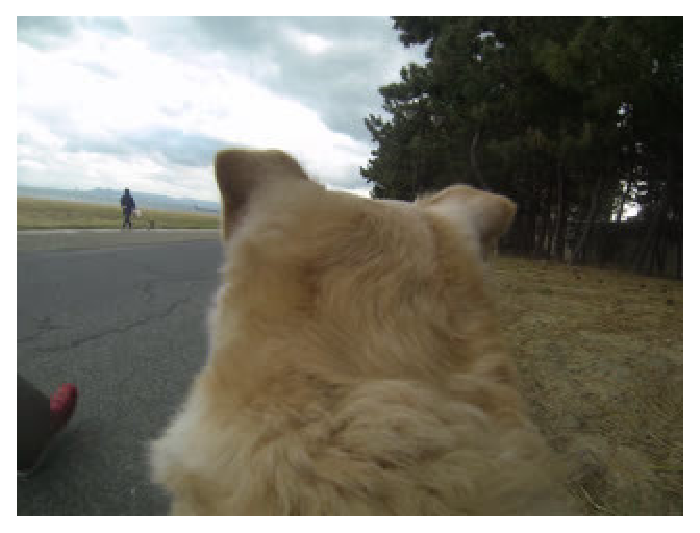
\includegraphics[clip, width=1.7cm]{./Figures/KL001.eps}
       \hspace{0.3cm} { }
      \end{center}
     \end{minipage}
     \begin{minipage}{0.18\hsize}
      \begin{center}
       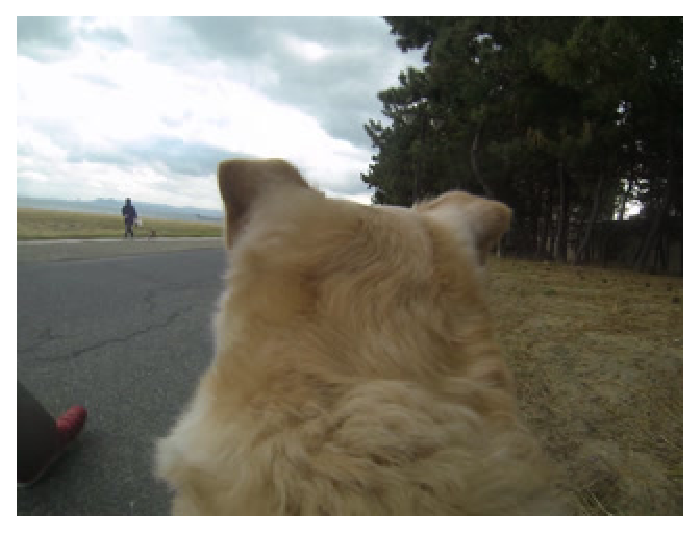
\includegraphics[clip, width=1.7cm]{./Figures/KL002.eps}
       \hspace{0.3cm} { }
      \end{center}
     \end{minipage}
     \begin{minipage}{0.18\hsize}
      \begin{center}
       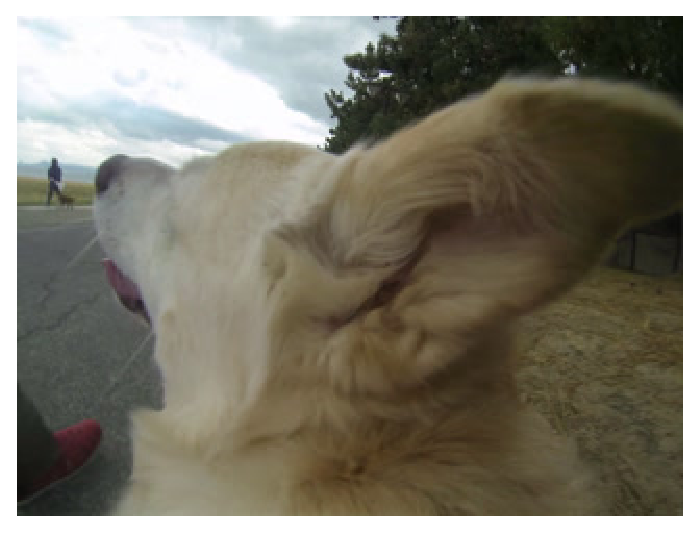
\includegraphics[clip, width=1.7cm]{./Figures/KL003.eps}
       \hspace{0.1cm} {Look\_at\_Left}
      \end{center}
     \end{minipage}
     \begin{minipage}{0.18\hsize}
      \begin{center}
       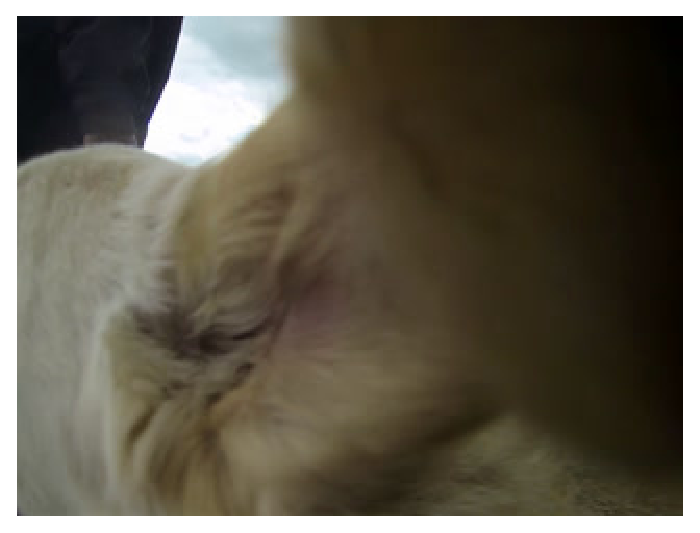
\includegraphics[clip, width=1.7cm]{./Figures/KL004.eps}
       \hspace{1.3cm} { }
      \end{center}
     \end{minipage}
     \begin{minipage}{0.18\hsize}
      \begin{center}
       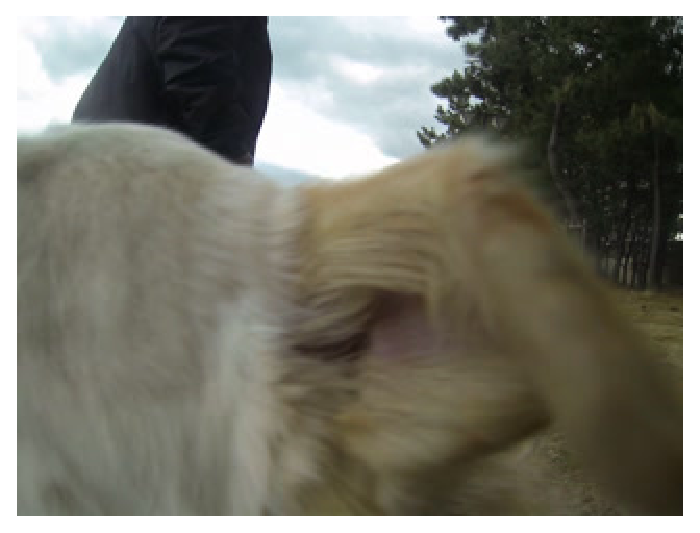
\includegraphics[clip, width=1.7cm]{./Figures/KL005.eps}
       \hspace{1.6cm} { }
      \end{center}
     \end{minipage}

    \end{tabular}
    \caption{DogCentric Activity Dataset}
    \label{DCAD_img}
%  \end{center}
\end{figure}

\section{サイバーレスキュー犬 訓練データセット}
サイバーレスキュー犬訓練データセットは,訓練されているレスキュー犬に,専用の計測スーツを着用させ収集したデータセットである.現在も作成中であり,完成していないデータを含めた全てを使用することは困難である.そのため,本研究ではその一部の提供されたデータをこれとして取り扱うものとする.
これは約2分から20分の7本の音声付き動画からなり,犬の一人称視点動画に加えてハンドラー視点動画,レスキュー犬とハンドラーを映す第三者視点動画が含まれる.本研究では犬の一人称視点動画のみを用いて推定を行う.
総時間は57分40秒,秒間フレーム数は29.97,総フレーム数は103696枚である.分類クラスそれぞれについて時間範囲を指定する形で動画にアノテーションがされており,複数のクラスが同時刻に重なるマルチラベルデータセットである.犬一人称、ハンドラー視点、第三者視点毎にそれぞれラベル付けされているが、アノテーション情報に関してはでは全てを用いて学習を行った.

\subsection{分類クラス詳細}
\subsubsection{bark}
被災者を発見し,かつ吠えている状態.わかりやすい音声的特徴があり,固有の画面揺れが生じる.
\subsubsection{cling}
臭いに対し,鼻を近づけ嗅いでいる状態.sniffのより詳細な状態であり,clingがラベル付される際はsniffと必ず重複する.
\subsubsection{command}
ハンドラーからの働きかけのある状態.待て/行け等の口頭指示,褒め,指差し指示など状況が多様.
\subsubsection{eat-drink}
何かを食べている/飲んでいる状態.訓練において被災者発見に対する成功報酬に餌が与えられる他,草を食む,地面/川の水を飲むなど状況が多様.
\subsubsection{look at handler}
犬がハンドラーを見ている状態.
\subsubsection{run}
走っている状態.walk-trotと比較すると,画面に浮遊感があり,揺れや音が激しい.
\subsubsection{see victim}
カメラに被災者が映った状態.
\subsubsection{shake}
犬が激しく体を震わせている状態.振動に合わせてカラカラカラとカメラの揺れる音がする.
\subsubsection{sniff}
臭いを嗅いでいる状態.探査に対するやる気などを測る一つに指標になる.地面などに鼻を近づけている状態だけでなく,浮遊臭を嗅いでいる際も含む.
\subsubsection{stop}
足を運んでいない状態.その場での足踏みは含む.方向転換は含まない.画面の動き情報が少なく特徴的である.
\subsubsection{walk-trot}
歩いており、runではない状態.
\subsection{データ整形}
本研究では,フレーム毎にラベルを対応づけた際のラベルのないフレームなどを排除し,過学習を防ぐ目的で6fpsとして整形したデータを用いた.
そのため,学習および評価に使った総フレーム数は14581枚となった.この範囲でラベル付けされた回数をクラス毎に~表\ref{cyberdataset_label}に示す.
画像のみでのクラス的特徴の図示は困難であるため、整形した動画的特徴,音声的特徴とをそれぞれ~図\ref{cyberdataset_img}に示す.
\begin{table}[tb]
 \centering
 \caption{サイバーレスキュー犬 訓練データセット 利用範囲内での出現回数}\label{cyberdataset_label}
 \scalebox{1.00}[1.00]{
  \begin{tabular}{|l||c|c|c|c|c|c|c|c|c|c|c|}
   \hline \hline
   ラベル & bark&cling&command&eat-drink&look at bandler&run&see victim&shake&sniff&stop&walk-trot \\ \hline
   出現回数& 1744& 1127&   2439&      343&           2011& 98&      1549&  239& 7719&6384&     8764 \\ \hline
  \end{tabular}
 }

\end{table}

\begin{figure}[htbp]
    \begin{tabular}{c}
     % 0
      \begin{minipage}{0.18\hsize}
        \begin{center}
          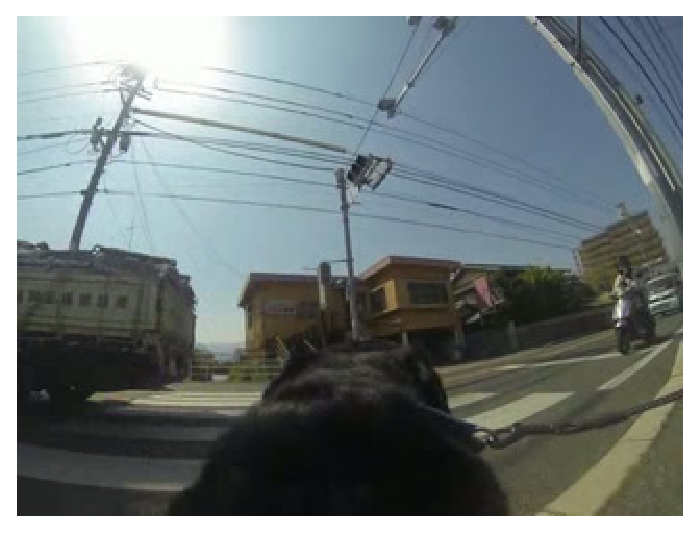
\includegraphics[clip, width=1.7cm]{./Figures/HC005.eps}
          \hspace{0.3cm} { }
        \end{center}
      \end{minipage}
      \begin{minipage}{0.18\hsize}
        \begin{center}
          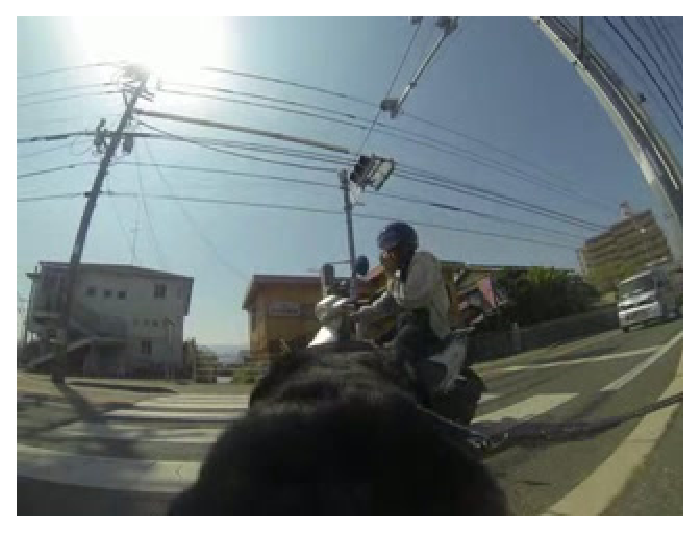
\includegraphics[clip, width=1.7cm]{./Figures/HC006.eps}
          \hspace{0.3cm} { }
        \end{center}
      \end{minipage}

      % 2
      \begin{minipage}{0.18\hsize}
        \begin{center}
          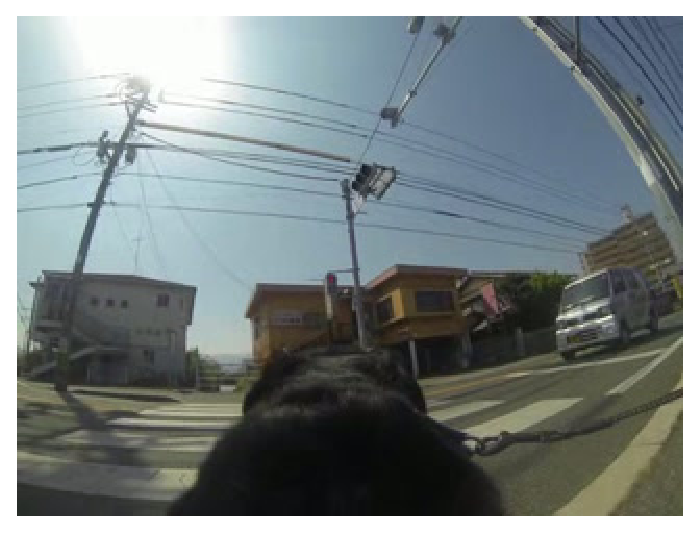
\includegraphics[clip, width=1.7cm]{./Figures/HC007.eps}
          \hspace{0.0cm} {Car}
        \end{center}
      \end{minipage}

      % 4
      \begin{minipage}{0.18\hsize}
        \begin{center}
          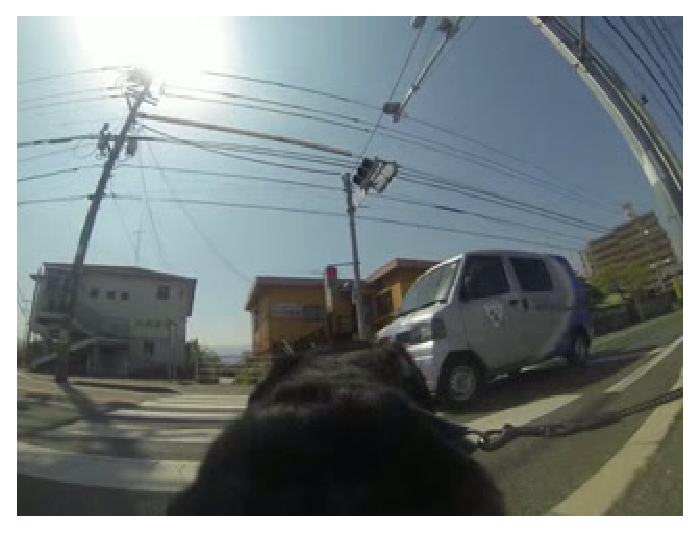
\includegraphics[clip, width=1.7cm]{./Figures/HC008.eps}
          \hspace{0.1cm} { }
        \end{center}
      \end{minipage}
      % 5
      \begin{minipage}{0.18\hsize}
        \begin{center}
          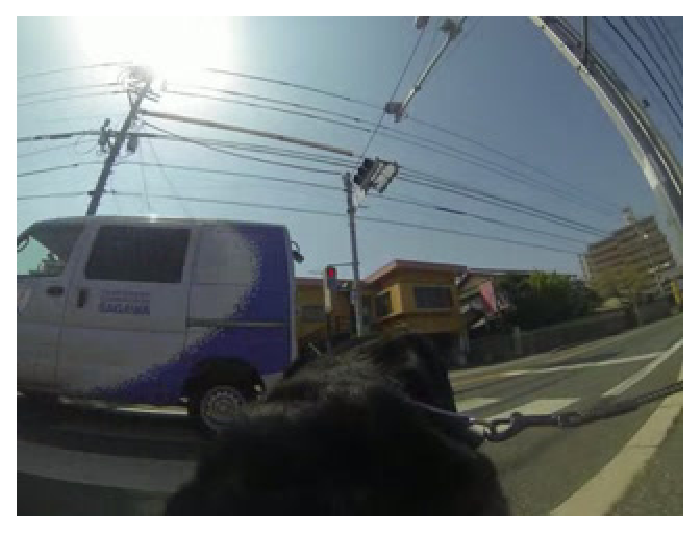
\includegraphics[clip, width=1.7cm]{./Figures/HC009.eps}
          \hspace{0.2cm} { }
        \end{center}
      \end{minipage}
\\
     \begin{minipage}{0.18\hsize}
      \begin{center}
       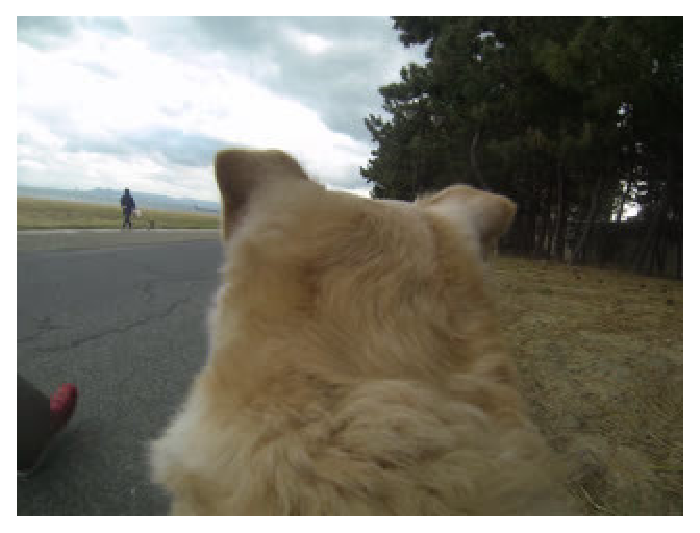
\includegraphics[clip, width=1.7cm]{./Figures/KL001.eps}
       \hspace{0.3cm} { }
      \end{center}
     \end{minipage}
     \begin{minipage}{0.18\hsize}
      \begin{center}
       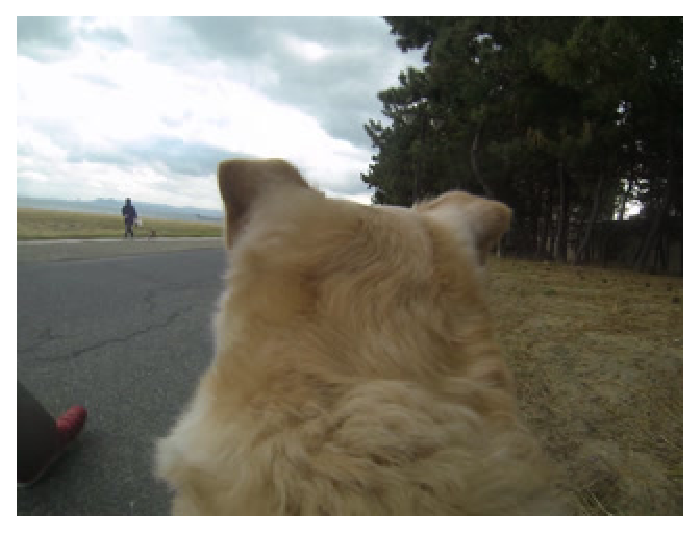
\includegraphics[clip, width=1.7cm]{./Figures/KL002.eps}
       \hspace{0.3cm} { }
      \end{center}
     \end{minipage}
     \begin{minipage}{0.18\hsize}
      \begin{center}
       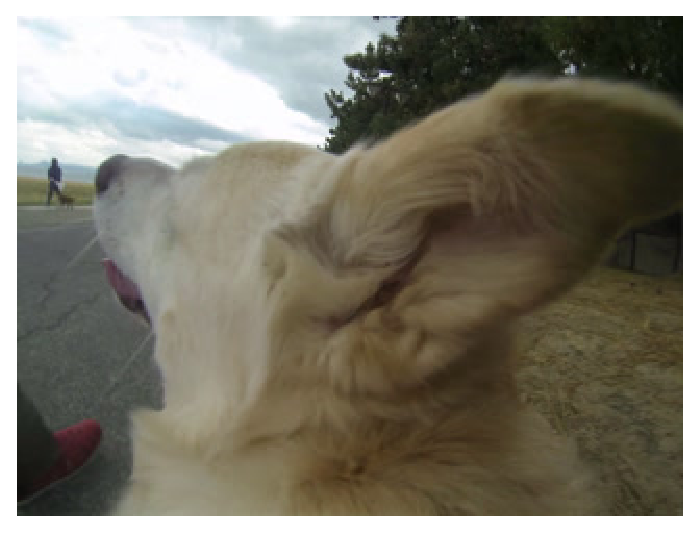
\includegraphics[clip, width=1.7cm]{./Figures/KL003.eps}
       \hspace{0.1cm} {Look\_at\_Left}
      \end{center}
     \end{minipage}
     \begin{minipage}{0.18\hsize}
      \begin{center}
       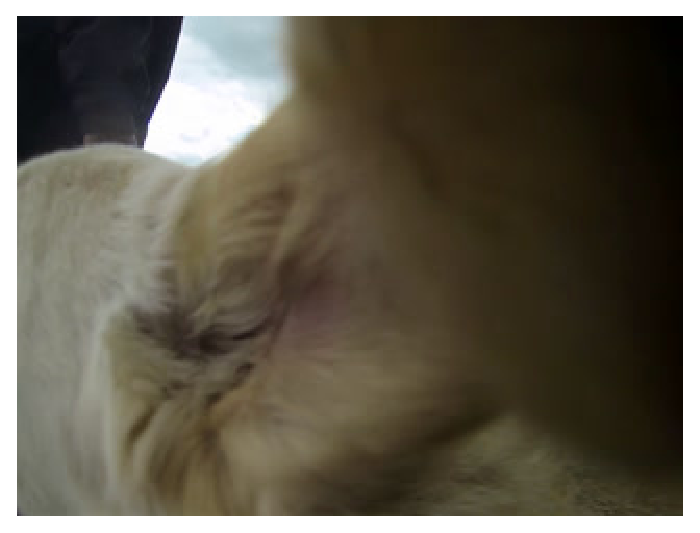
\includegraphics[clip, width=1.7cm]{./Figures/KL004.eps}
       \hspace{1.3cm} { }
      \end{center}
     \end{minipage}
     \begin{minipage}{0.18\hsize}
      \begin{center}
       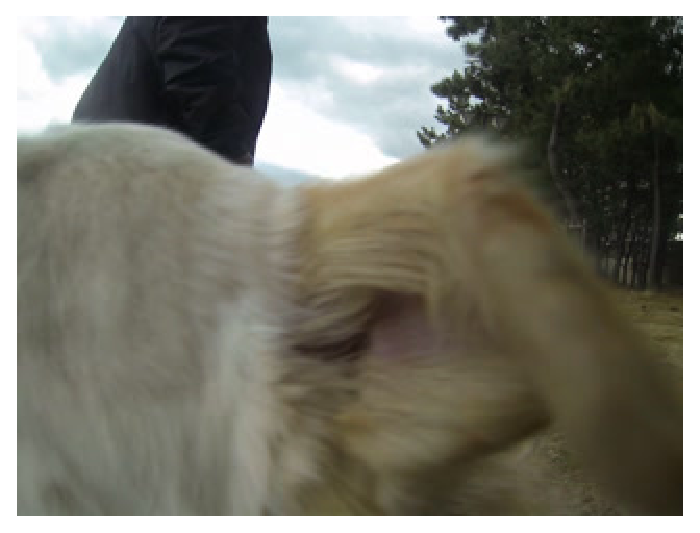
\includegraphics[clip, width=1.7cm]{./Figures/KL005.eps}
       \hspace{1.6cm} { }
      \end{center}
     \end{minipage}

    \end{tabular}
    \caption{サイバーレスキュー犬訓練データセット}
    \label{cyberdataset_img}
\end{figure}
%    \caption{サイバーレスキュー犬訓練データセット オプティカルフロー画像}
%    \label{cyberdataset_optical}
%    \caption{サイバーレスキュー犬訓練データセット サウンドスペクトログラム}
%    \label{cyberdataset_spectrum}


